\section{Risultati}
Dopo lo studio e l'analisi di ogni metodologia di rilievo dendrometrico, è possibile trarre alcune considerazioni.\\
La particella ovest si presenta come una pineta, in cui sono presenti maggiormente Pinus pinea, Pinus pinaster e qualche latifoglia (es Quercus liex). Il bosco, che si estende per un'area di 2,24 ha, ha una struttura biplana.\\
La particella est invece, si presenta come una pineta composta solamente da Pinus pinea. La struttura di questo bosco è monoplana, e si estende per un'area di 2,72 ha.
\subsection{Cavallettamento totale}
\subsubsection*{Particella ovest}
Come si può notare dall'istogramma \autoref{fig:cavallettamento_ovest} del cavallettamento  totale ovest, la specie arborea maggiormente presente è il pino domestico, tranne nella classe dei 20 cm, dove il pino marittimo ha una numerosità superiore. In tutte le classi, le latifoglie sono presenti in numerosità e grandezze minori.
\begin{figure}[H]
    \centering
    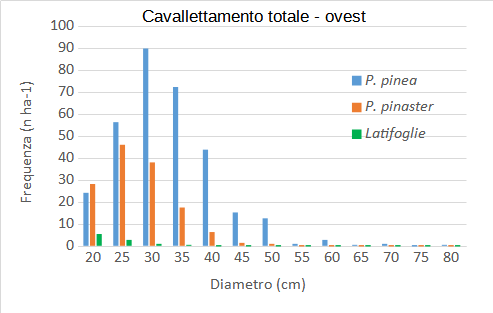
\includegraphics[width=0.7 \textwidth]{immagini/cav-tot-ovest.png}
    \caption{Distribuzione per classe diametrica, e per specie arborea, del popolamento della particella ovest, ricavata mediante cavallettamento totale.}
    \label{fig:cavallettamento_ovest}
\end{figure}

\begin{table}[H]
\caption{Distribuzione delle frequenze degli alberi, riferita all'area di un ettaro, della particella ovest.}
\centering
\begin{tabular}{ccccc}
\toprule
Classe & \textit{P. pinea} & \textit{P. pinaster} & Latifoglie & Totale \\
\midrule
20     & 24                & 28                   & 5          & 58     \\
25     & 56                & 46                   & 3          & 105    \\
30     & 90                & 38                   & 1          & 129    \\
35     & 72                & 17                   & 0          & 90     \\
40     & 44                & 6                    & 0          & 50     \\
45     & 15                & 1                    & 0          & 17     \\
50     & 13                & 1                    & 0          & 13     \\
55     & 1                 & 0                    & 0          & 1      \\
60     & 3                 & 0                    & 0          & 3      \\
65     & 0                 & 0                    & 0          & 0      \\
70     & 1                 & 0                    & 0          & 1      \\
75     & 0                 & 0                    & 0          & 0      \\
80     & 0                 & 0                    & 0          & 0     \\
\bottomrule
\end{tabular}
\label{tab:tab_freq_cav_ovest}
\end{table}

\begin{table}[H]
  \caption{Parametri ricavati dallo studio della particella ovest}
    \centering
    \begin{tabular}{ccccc}
     \toprule
       & Pinus pinea & Pinus pinaster &  Latifoglie & Totale  \\
       \midrule
        $N$ tot & 715 & 309 & 21 & 1045\\
        $\frac{N}{ha}$ & 319 & 138 & 9 & 467\\
        $G$  tot $(m^2)$ & 64,5 & 19,5 & 0,9 & 84,8\\
        $\frac{G}{ha}$ $(\frac{m^3}{ha})$ & 28,8 & 8,7 & 0,4 & 37,8\\
        $g$ medio $(cm^2)$ & 901 & 630 & 411 & 811\\
        diametro medio $(cm)$ & 34 & 28 & 23 & 32\\
       \bottomrule
        \end{tabular}
    \label{tab:tab_cav_ovest}
\end{table}


\subsubsection*{Particella est}
Grazie all'istogramma \autoref{fig:cavallettamento_est}, ovvero la rappresentazione grafica della distribuzione della particella est, si può notare come la classe diametrica più rappresentata sia quella dei 25 cm.
\begin{figure}[H]
    \centering
    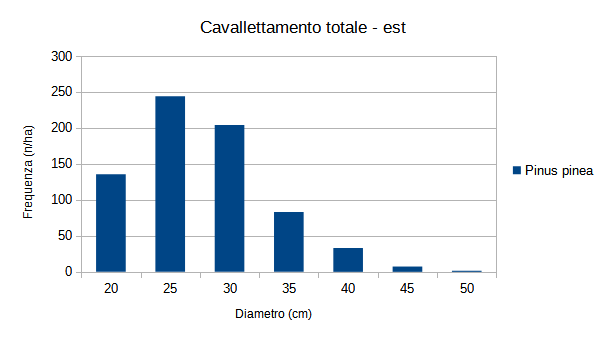
\includegraphics[width=0.7 \textwidth]{immagini/cav-tot-est.png}
    \caption{Distribuzione per classe diametrica del popolamento di Pinus pinea della particella est, ricavata mediante cavallettamento totale.}
    \label{fig:cavallettamento_est}
\end{figure}
\begin{table}[H]
\caption{Distribuzione delle frequenze degli alberi, riferita all'area di un ettaro, della particella est, con valori ricavati mediante cavallettamento totale.}
\centering
\begin{tabular}{cc}
\toprule
Classe & Pinus pinea \\
\midrule
20     & 136         \\
25     & 244         \\
30     & 204         \\
35     & 83          \\
40     & 33          \\
45     & 7           \\
50     & 1           \\ 
\bottomrule
\end{tabular}
\label{tab:tab_freq_cav_est}
\end{table}

\begin{table}[H]
  \caption{Parametri ricavati dallo studio della particella est}
    \centering
    \begin{tabular}{cc}
     \toprule
       & Pinus pinea \\
       \midrule
        $N$ tot & 1928 \\
        $\frac{N}{ha}$ & 709 \\
        $G$ tot $(m^2)$ & 120 \\
        $\frac{G}{ha}$ $(\frac{m^3}{ha})$ & 44\\
        $g$ medio $(cm^2)$ & 620 \\
        diametro medio $(cm)$ & 28\\
       \bottomrule
        \end{tabular}
    \label{tab:tab_cav_est}
\end{table}

%%%%%%%%%%%%%%%%%%%%%%%%%%%%%%%%%%%%%%%%%%%%%%%%%%%%%%%%%%%%%%%%%%%%%%%%%%%
\subsection{Aree di saggio con raggio fisso}
\subsubsection*{Particella ovest}
Utilizzando l'istogramma \autoref{fig:aree_saggio_ovest} e la tabella \autoref{tab:tab_areesaggio_ovest}, è possibile comprendere la composizione e la frequenza della particella ovest.\\
La maggior parte degli alberi presenti appartiene alla specie del pino domestico, a eccezione della classe del 20 cm, dove c'è una maggiore presenza del pino marittimo.\\
In tutte le classi diametriche le conifere sono in minore numerosità.
\begin{figure}[H]
    \centering
    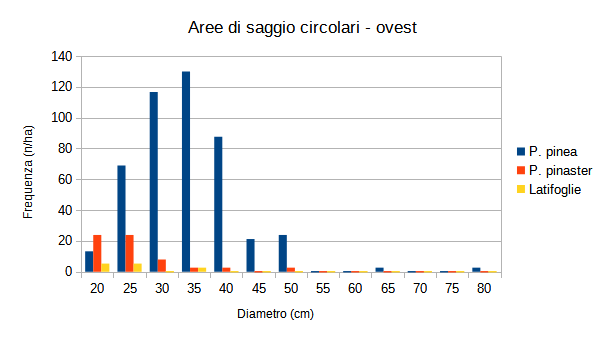
\includegraphics[width=0.7 \textwidth]{immagini/aree-saggio-ovest.png}
    \caption{Distribuzione per classe diametrica, e per specie arborea, del popolamento della particella ovest, ricavata mediante aree di saggio circolari di raggio 10 m. }
    \label{fig:aree_saggio_ovest}
\end{figure}

\begin{table}[H]
\caption{Distribuzione delle frequenze degli alberi, riferita all'area di un ettaro, della particella ovest.}
\centering
\begin{tabular}{ccccc}
\toprule
Classe & \textit{P. pinea} & \textit{P. pinaster} & Latifoglie \\
\midrule
20     & 13                & 24                   & 5          \\
25     & 69                & 24                   & 5          \\
30     & 117               & 8                    & 0          \\
35     & 130               & 3                    & 3          \\
40     & 88                & 3                    & 0          \\
45     & 21                & 0                    & 0          \\
50     & 24                & 3                    & 0          \\
55     & 0                 & 0                    & 0          \\
60     & 0                 & 0                    & 0          \\
65     & 3                 & 0                    & 0          \\
70     & 0                 & 0                    & 0          \\
75     & 0                 & 0                    & 0          \\
80     & 3                 & 0                    & 0         \\
\bottomrule
\end{tabular}
\label{tab:tab_freq_aree_saggio_ovest}
\end{table}

\begin{table}[H]
  \caption{Parametri ricavati dallo studio della particella ovest}
    \centering
    \begin{tabular}{ccccc}
     \toprule
       & Pinus pinea & Pinus pinaster &  Latifoglie & Totale  \\
       \midrule
        $N$ tot & 176 & 24 & 5 & 205\\
        $\frac{N}{ha}$ media & 467 & 64 & 13 & 544\\
         $G$ tot $(m^2)$ & 17,3 & 1.3 & 0.2 & 18.9\\
        $\frac{G}{ha}$ media $(\frac{m^3}{ha})$ & 46 & 4 & 1 & 50\\
        $g$ medio $(cm^2)$ & 1096 & 609 & 484 & 969\\
        diametro medio  $(cm)$ & 37 & 28 & 25 & 35\\
        conf. diametro medio $(cm)$ & 5 & 3 & 1 & 9 \\
       \bottomrule
        \end{tabular}
    \label{tab:tab_areesaggio_ovest}
\end{table}

\subsubsection*{Particella est}
Utilizzando le aree di saggio sottostanti, è possibile comprendere la composizione del popolamento della particella est. La maggioranza degli individui è rappresentata da alberi appartenenti alla classe dei 25 cm di diametro.

\begin{figure}[H]
    \centering
    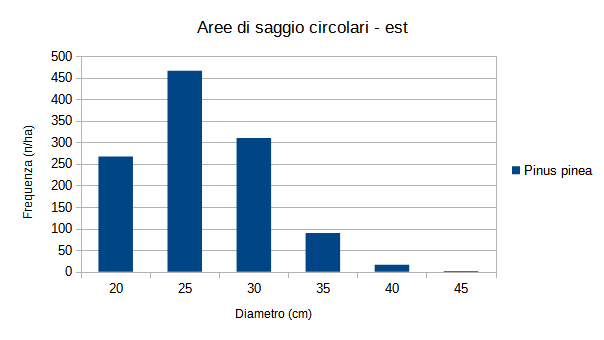
\includegraphics[width=0.7 \textwidth]{immagini/aree-saggio-est.png}
    \caption{Distribuzione per classe diametrica, del popolamento di Pinus pinea della particella est, ricavata mediante aree di saggio circolari di raggio 10 m. }
    \label{fig:aree_saggio_est}
\end{figure}

\begin{table}[H]
\caption{Distribuzione delle frequenze degli alberi, riferita all'area di un ettaro, della particella est, con valori ricavati da aree di saggio circolari.}
\centering
\begin{tabular}{cc}
\toprule
Classe & Pinus pinea \\
\midrule
20     & 267         \\
25     & 466         \\
30     & 310         \\
35     & 90         \\
40     & 16          \\
45     & 2         \\
\bottomrule
\end{tabular}
\label{tab:tab_area_saggio_est}
\end{table}

\begin{table}[H]
  \caption{Parametri ricavati dallo studio della particella est}
    \centering
    \begin{tabular}{cc}
     \toprule
       & Pinus pinea  \\
       \midrule
        $N$ tot & 578\\
        $\frac{N}{ha}$ media & 1150 \\
         $G$ tot $(m^2)$ & 32 \\
        $\frac{G}{ha}$ media $(\frac{m^3}{ha})$ & 63 \\
        $g$ medio $(cm^2)$ & 565 \\
        diametro medio  $(cm)$ & 27 \\
        conf. diametro medio $(cm)$ & 4 \\
       \bottomrule
        \end{tabular}
    \label{tab:tab_areesaggio_est}
\end{table}

%%%%%%%%%%%%%%%%%%%%%%%%%%%%%%%%%%%%%%%%%%%%%%%%%%%%%%%%%%%%%%%%%%%%%%%%
\subsection{Aree relascopiche diametriche}
\subsubsection*{Particella ovest}
Anche mediante questo metodo di rilievo, si può notare dal grafico \autoref{fig:aree-relascopiche-ovest} come il popolamento di P. pinea sia più numeroso rispetto alle altre due specie arboree. La frequenza maggiore di pino domestico è all'interno della classe dei 30 cm.\\
\begin{figure}[H]
    \centering
    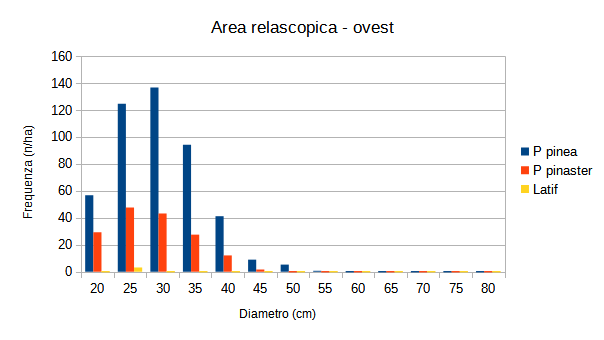
\includegraphics[width=0.7 \textwidth]{immagini/aree-relascopiche-ovest.png}
    \caption{Distribuzione per classe diametrica, e per specie arborea, del popolamento della particella ovest, ricavata mediante metodo delle aree relascopiche.}
    \label{fig:aree-relascopiche-ovest}
\end{figure}

\begin{table}[H]
\caption{Distribuzioni delle frequenze, a ettaro, degli individui della particella ovest, suddivise per classi diametriche.}
\centering
\begin{tabular}{cccc}
\toprule
Classe & P pinea & P pinaster & Latif \\
\midrule
20     & 57      & 29         & 0     \\
25     & 125     & 48         & 3     \\
30     & 137     & 43         & 0     \\
35     & 94      & 28         & 0     \\
40     & 41      & 12         & 0     \\
45     & 9       & 2          & 0     \\
50     & 5       & 0          & 0     \\
55     & 1       & 0          & 0     \\
60     & 0       & 0          & 0     \\
65     & 0       & 0          & 0     \\
70     & 0       & 0          & 0     \\
75     & 0       & 0          & 0     \\
80     & 0       & 0          & 0    \\
\bottomrule
\end{tabular}
\label{tab:tab_freq_rel_ovest}
\end{table}

\begin{table}[H]
  \caption{Parametri ricavati dallo studio della particella ovest}
    \centering
     \begin{tabular}{ccccc}
     \toprule
       & Pinus pinea & Pinus pinaster &  Latifoglie & Totale  \\
       \midrule
        $N$ tot & 206 & 64 & 1 & 270\\
        $\frac{N}{ha}$ media & 468 & 161 & 3 & 633\\
         $G$ tot $(m^2)$ & 18 & 4.9 & 0.05 & 23 \\
        $\frac{G}{ha}$ media $(\frac{m^3}{ha})$ & 34 & 11 & 0.1 & 45\\
        $g$ medio $(cm^2)$ & 766 & 685 & 531 & 722\\
        diametro medio  $(cm)$ & 31 & 29 & 26 & 30\\
        conf. diametro medio $(cm)$ & 3 & 4 & 1 & 4 \\
       \bottomrule
        \end{tabular}
    \label{tab:tab_relascopica_ovest}
\end{table}

\subsubsection*{Particella est}
Grazie alla rappresentazione grafica, mediante istogramma, o alle indicazioni tabellari, è possibile comprendere la distribuzione del popolamento in esame. Se ne ricava l'informazione della classe più numerosa, ovvero quella dei 25 cm.
\begin{figure}[H]
    \centering
    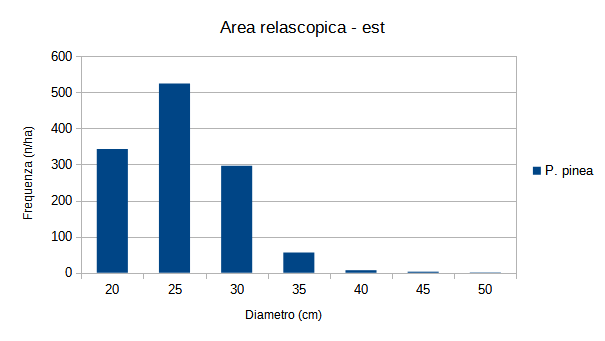
\includegraphics[width=0.7 \textwidth]{immagini/aree-relascopiche-est.png}
    \caption{Distribuzione per classe diametrica, del popolamento della particella est, ricavata mediante metodo delle aree relascopiche.}
    \label{fig:aree-relascopiche-est}
\end{figure}

\begin{table}[H]
\caption{Distribuzione delle frequenze degli alberi, riferita all'area di un ettaro, della particella est, con valori ricavati mediante metodo relascopico.}
\centering
\begin{tabular}{cc}
\toprule
Classe & Pinus pinea \\
\midrule
20     & 343      \\
25     & 524      \\
30     & 296      \\
35     & 56       \\
40     & 7        \\
45     & 3        \\
50     & 1        \\
55     & 0        \\
60     & 0        \\
65     & 0     \\
\bottomrule
\end{tabular}
\label{tab:tab_freq_relascopia_est}
\end{table}

\begin{table}[H]
  \caption{Parametri ricavati dallo studio della particella est}
    \centering
    \begin{tabular}{cc}
     \toprule
       & Pinus pinea  \\
       \midrule
        $N$ tot & 511 \\
        $\frac{N}{ha}$ media & 1229 \\
         $G$ tot $(m^2)$ & 30 \\
        $\frac{G}{ha}$ media $(\frac{m^3}{ha})$ & 64 \\
        $g$ medio $(cm^2)$ & 527 \\
        diametro medio  $(cm)$ & 26 \\
        conf. diametro medio $(cm)$ & 0,9 \\
       \bottomrule
        \end{tabular}
    \label{tab:tab_relascopia_est}
\end{table}



%%%%%%%%%%%%%%%%%%%%%%%%%%%%%%%%%%%%%%%%%%%%%%%%%%%%%%%%%%%%%%%%%%%%%%%%%%%
\subsection{Altezze e curve diametriche}
\subsubsection*{Particella ovest}
Nella particella ovest, essendoci tre diverse specie arboree, c'è la necessità di ricavare i valori di tre altezze medie.\\
\begin{figure}[H]
    \centering
    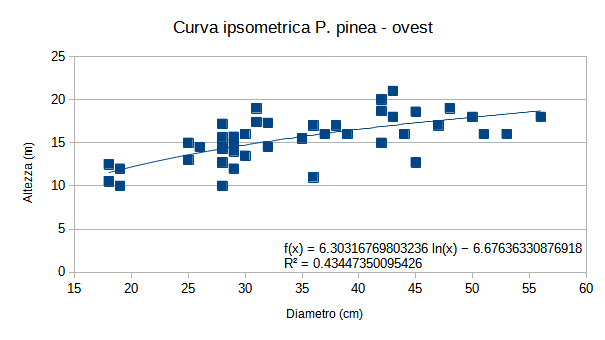
\includegraphics[width=0.7 \textwidth]{immagini/ipsom_pinea_ovest.png}
    \caption{Curva ipsometrica di P. pinea, della particella ovest.}
    \label{fig:ipsom_pinea_ovest}
\end{figure}
Introducendo nella formula della curva interpolante il diametro medio della specie, che è $33,77$ cm, l'altezza media risultante sarà $15.5$ m.
\begin{figure}[H]
    \centering
    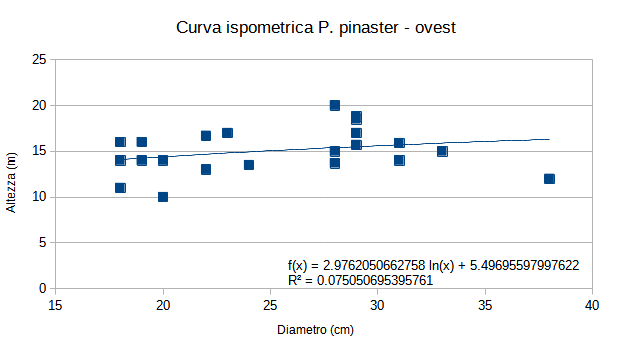
\includegraphics[width=0.7 \textwidth]{immagini/ipsom_pinaster_ovest.png}
    \caption{Curva ipsometrica di P. pinaster, della particella ovest.}
    \label{fig:ipsom_pinaster_ovest}
\end{figure}
Introducendo nella formula della curva logaritmica interpolante il valore del diametro medio della specie, presente nel popolamento, ovvero $28,32$ cm, l'altezza risultante sarà $15,45$ m.\\
Nel caso delle latifoglie, si estrae il valore mediano della serie delle altezze, che è $14$ m.\\
Come anticipato precedentemente, la particella ovest può essere definita come una pineta biplana, essendoci una differenza di altezze all'interno di essa.
\subsubsection*{Particella est}
Nella particella est, essendoci solamente una specie arborea, è sufficiente calcolare una sola altezza media.
\begin{figure}[H]
    \centering
    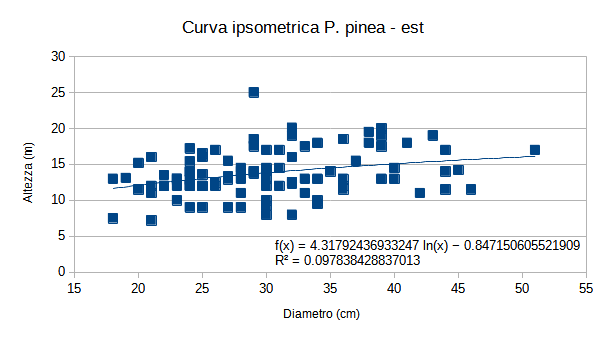
\includegraphics[width=0.7 \textwidth]{immagini/ipsom_pinea_est.png}
    \caption{Curva ipsometrica di P. pinea, della particella est.}
    \label{fig:ipsom_pinea_est}
\end{figure}
Introducendo nella formula della curva logaritmica interpolante il valore del diametro medio dei soggetti del popolamento, ovvero $28,1$ cm, l'altezza risultante sarà $13.6$ m.\\
Ne risulta che, l'altezza media del popolamento della particella est è minore di quello della particella ovest.
%%%%%%%%%%%%%%%%%%%%%%%%%%%%%%%%%%%%%%%%%%%%%%%%%%%%%%%%%%%%%%%%%%%%%%%%%%%
\subsection{Volumi}
\subsubsection*{Particella ovest}
Com'è possibile notare dalle due tabelle sottostanti, la classe diametrica con il maggiore volume di biomassa è quella dei 35 cm, poco superiore di quella dei 30 cm.
\begin{table}[H]
\caption{Volumi (in $\frac{m^3}{ha}$), del popolamento ovest, suddivisi per specie arborea e classi diametriche, secondo le tavole Ravenna.}
\centering
\begin{tabular}{ccccc}
\toprule
Diametro & P. pinea & P. pinaster & Latif & Totale \\
\midrule
20       & 3.67    & 4.29       & 1.18  & 9.14   \\
25       & 15.93   & 13.02      & 0.92  & 29.87  \\
30       & 40.18   & 16.99      & 0.44  & 57.62  \\
35       & 47.25   & 11.38      & 0.30  & 58.93  \\
40       & 37.58   & 5.37       & 0.00  & 42.95  \\
45       & 16.16   & 1.43       & 0.00  & 17.58  \\
50       & 15.88   & 1.13       & 0.00  & 17.01  \\
55       & 1.32    & 0.00       & 0.00  & 1.32   \\
60       & 4.50    & 0.00       & 0.00  & 4.50   \\
65       & 0.84    & 0.00       & 0.00  & 0.84   \\
70       & 1.87    & 0.00       & 0.00  & 1.87   \\
75       & 0.00    & 0.00       & 0.00  & 0.00   \\
80       & 1.12    & 0.00       & 0.00  & 1.12   \\
\midrule
&&&&  242,8\\
\bottomrule
\end{tabular}
\label{tab:volumi_ravenna_ettaro_ovest}
\end{table}

\begin{table}[H]
\caption{Volumi (in $\frac{m^3}{ha}$) del popolamento, suddivisi per specie arborea e classi diametriche, secondo le tavole Tabacchi.}
\centering
\begin{tabular}{ccccc}
\toprule
Diametro & P pinea & P pinaster & Latif & Totale \\
\midrule
     20    & 4.83    & 6.31       & 1.25  & 12.38  \\
   25  & 19.66   & 16.77      & 0.97  & 37.40  \\
   30      & 49.00   & 20.59      & 0.46  & 70.05  \\
    35     & 57.30   & 13.21      & 0.31  & 70.83  \\
    40     & 47.70   & 6.34       & 0.00  & 54.05  \\
      45   & 21.89   & 1.76       & 0.00  & 23.64  \\
    50     & 23.11   & 1.47       & 0.00  & 24.58  \\
    55     & 2.06    & 0.00       & 0.00  & 2.06   \\
      60   & 7.59    & 0.00       & 0.00  & 7.59   \\
    65     & 1.52    & 0.00       & 0.00  & 1.52   \\
      70   & 3.62    & 0.00       & 0.00  & 3.62   \\
    75     & 0.00    & 0.00       & 0.00  & 0.00   \\
     80    & 2.46    & 0.00       & 0.00  & 2.46  \\
     \midrule
     &&&& 310,2\\
     \bottomrule
\end{tabular}
\end{table}

\subsubsection*{Particella est}
\begin{table}[H]
\caption{Volumi (in $\frac{m^3}{ha}$), del popolamento est, suddivisi per classi diametriche, secondo le tavole Ravenna.}
\centering
\begin{tabular}{cc}
\toprule
Diametro & P. pinea \\
\midrule
20       & 20,1    \\
25       & 69,1     \\
30       & 91,4     \\
35       & 54,2     \\
40       & 28,3    \\
45       & 7,5     \\
50       & 1,3  \\
\midrule
Totale & 272,5 \\
\bottomrule
\end{tabular}
\label{tab:volumi_ravenna_ettaro_est}
\end{table}

\begin{table}[H]
\caption{Volumi (in $\frac{m^3}{ha}$), del popolamento est, suddivisi per classi diametriche, secondo le tavole Tabacchi.}
\centering
\begin{tabular}{cc}
\toprule
Diametro & P. pinea \\
\midrule
20       & 27,0    \\
25       & 81,7     \\
30       & 104,4     \\
35       & 60,6    \\
40       & 32,7    \\
45       & 9,1    \\
50       & 1,6  \\
\midrule
Totale & 317,1 \\
\bottomrule
\end{tabular}
\label{tab:volumi_tabacchi_ettaro_est}
\end{table}